\chapter{Level One Trigger} % (fold)
\label{cha:level_one_trigger}
The CMS \Lone trigger system\cite{l1} is a pipelined dead-timeless system based on custom-built electronics.
The \Lone trigger is a combination of several sub systems.
\begin{itemize}
  \item Reginal Callorimeter (RCT).
  \item Global Muon Trigger (GMT).
  \item Global Callorimeter Trigger (GCT).
  \item Global Trigger (GT).
\end{itemize}

\textbf{Some stuff about each of the sub systems}

\section{GCT Hadronic triggers} % (fold)
\label{sec:gct_hadronic_triggers}
The global calorimeter trigger is responsible for forming hadronic jets in the central and forward sections of the hadronic 
calorimeters, there is a separate algorithm for forming hadronic $\tau$ jets. First 108 internal jets are formed and ordered, these 
jets are then used to calculate \HT and \MHT. The four highest energy jets then have their energy corrected, by passing though a
look up table which is dependent on \ET and \mETA, these jets are then passed to the Global Trigger so that the final trigger
decision can be made.

\textbf{THIS IS BY NO MEANS FINISHED, NEED TO DISCUSS IN DEPTH THE L1 JET FINDING AND THE PERFORMANCE AT LOW PU OF
 BOTH SETS OF CORRECTIONS. PERFORMANCE IN 2011 THEN MOVE ON TO WHY ITS IMPORTANT TO DO SOME SORT OF PILE UP
  CORRECTION. REMEMBER TO USE THE FOLLOWING IMAGE!!!}

\begin{figure}[htbp]
  \centering
    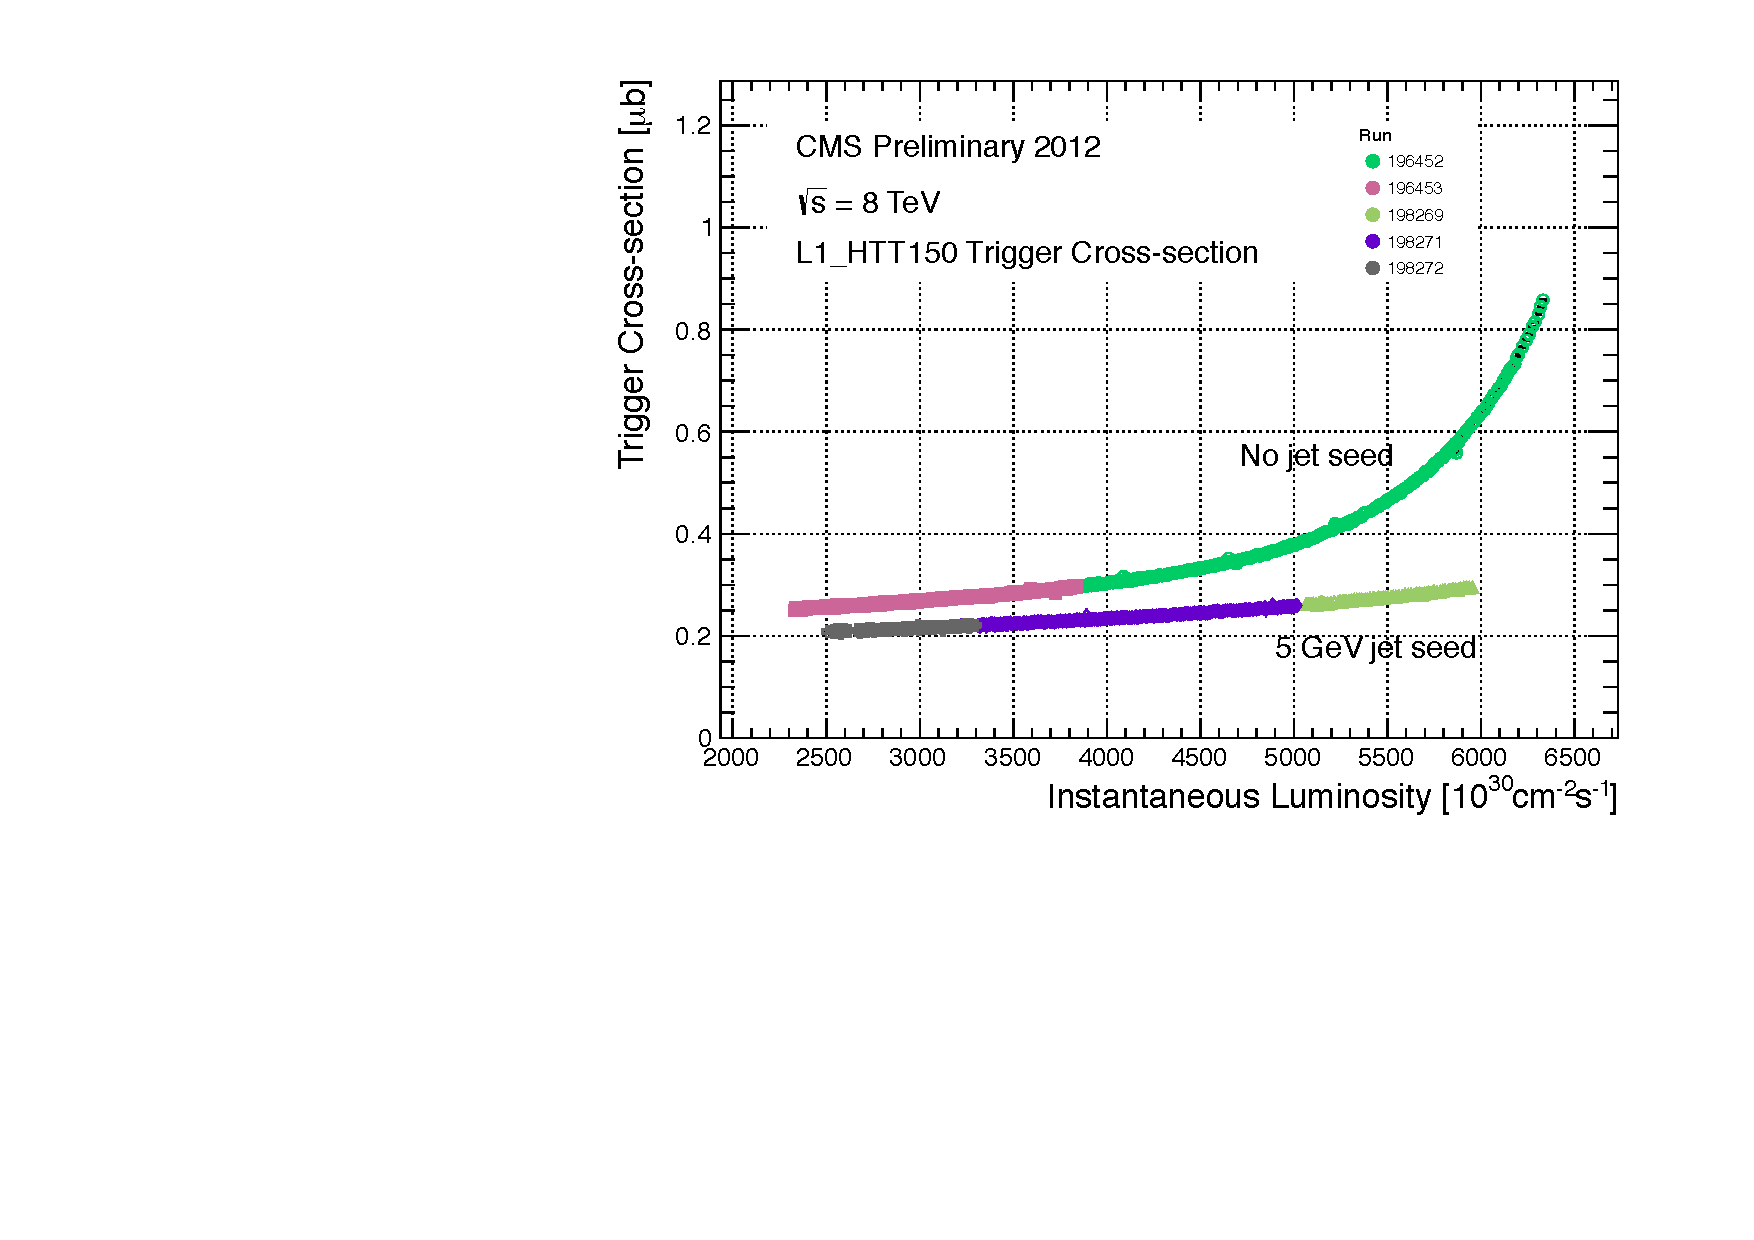
\includegraphics[width=ht]{figures/LoneTrigger/HTT150_pileup.pdf}
  \caption{caption}
  \label{fig:figures_LoneTrigger_HTT150_pileup}
\end{figure}


\subsection{Level-1 Trigger Jet Algorithm} % (fold)
\label{sec:Level-1 Trigger Jet Algorythm}
The jet finding algorithm \cite{gctcomm} at \Lone finds local maxima from $3\times3$ blocks
of trigger regions. The central trigger region
is required to have $E_{T}^{cen} \geq E_{T}^{surrounding}$, however there is no direct
requirement on the energy deposited in the central region.

\begin{figure}[htbp]
  \centering
    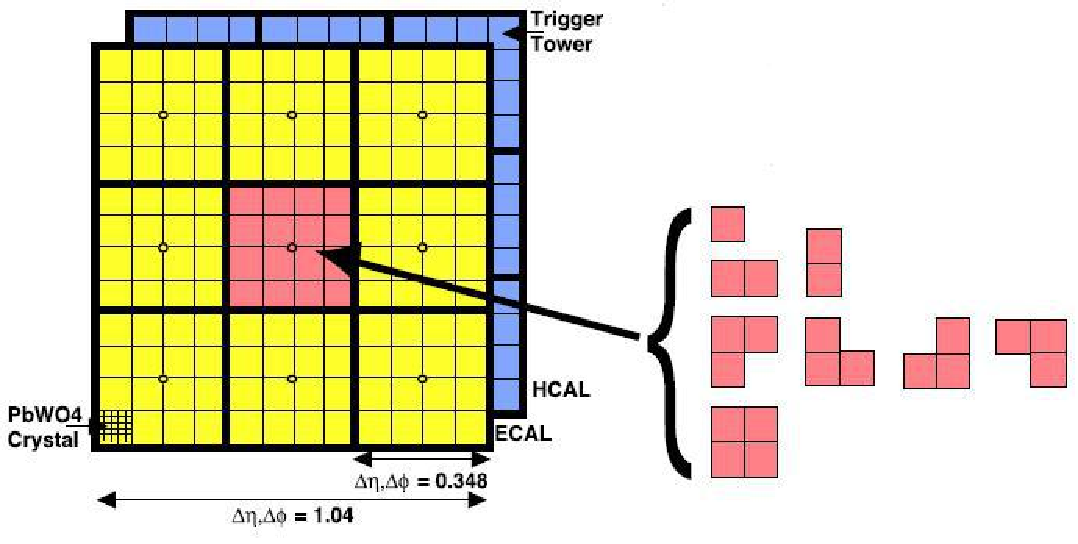
\includegraphics[width=\textwidth]{generated/LoneTrigger/level1jetalgo.pdf}
  \caption{graphic of \Lone jet algorithm}
  \label{fig:figures_level1jetalgo}
\end{figure}


Due to the lack of a requirement of a jet seed threshold, soft non-collimated jets, such as
those expected in a high pile up environment are found. Trigger decisions are then made using these pile up jets.

This is less of a problem for the single jet triggers which have a high $P_{T}$ threshold.
However the \HT triggers, where \HT = $\sum_{jets}E_{T}^{jet}$ and the requirement of \ET$^{jet} \geq $10 \GeV is made,
see a large increase in rate due to pile-up, this is due to the low energy threshold required for a jet to be added to the \HT sum.

To counteract the effect of pile up on trigger rate we study the effects of requiring a jet
seed threshold on the rate and efficiency of the individual jet and \HT triggers.

Figure~\ref{fig:figures_level1jetalgo} depicts 3$\times$3 trigger regions, each of which are built from 4$\times$4 trigger towers.
In this case the central region is the jet seed. The proposed change would require there to be a threshold energy in the seed
region.

a
The study of using jet seed thresholds of 2 and 5 \GeV is presented. The maximum energy of effected jets is 18 \GeV when 
requiring a seed of 2 \GeV and 45 \GeV when requiring a seed of 5 \GeV for jets made from $3\times3$ trigger regions, however 
some jets can include more than 9 trigger regions. The jet clustering is performed before the \Lone jets are corrected according 
to their \ET and $\eta$, hence the effects are manifested in trigger decisions for \Lone jets above 18 or 45 \GeV.



\begin{figure}[h!]
    \centering
    \subfigure[GCT jet $E_{T}$ distributions for the same events with a 0, 2 or 5 \GeV seed requirement.]{
          \label{fig:GCTrankRAW}
          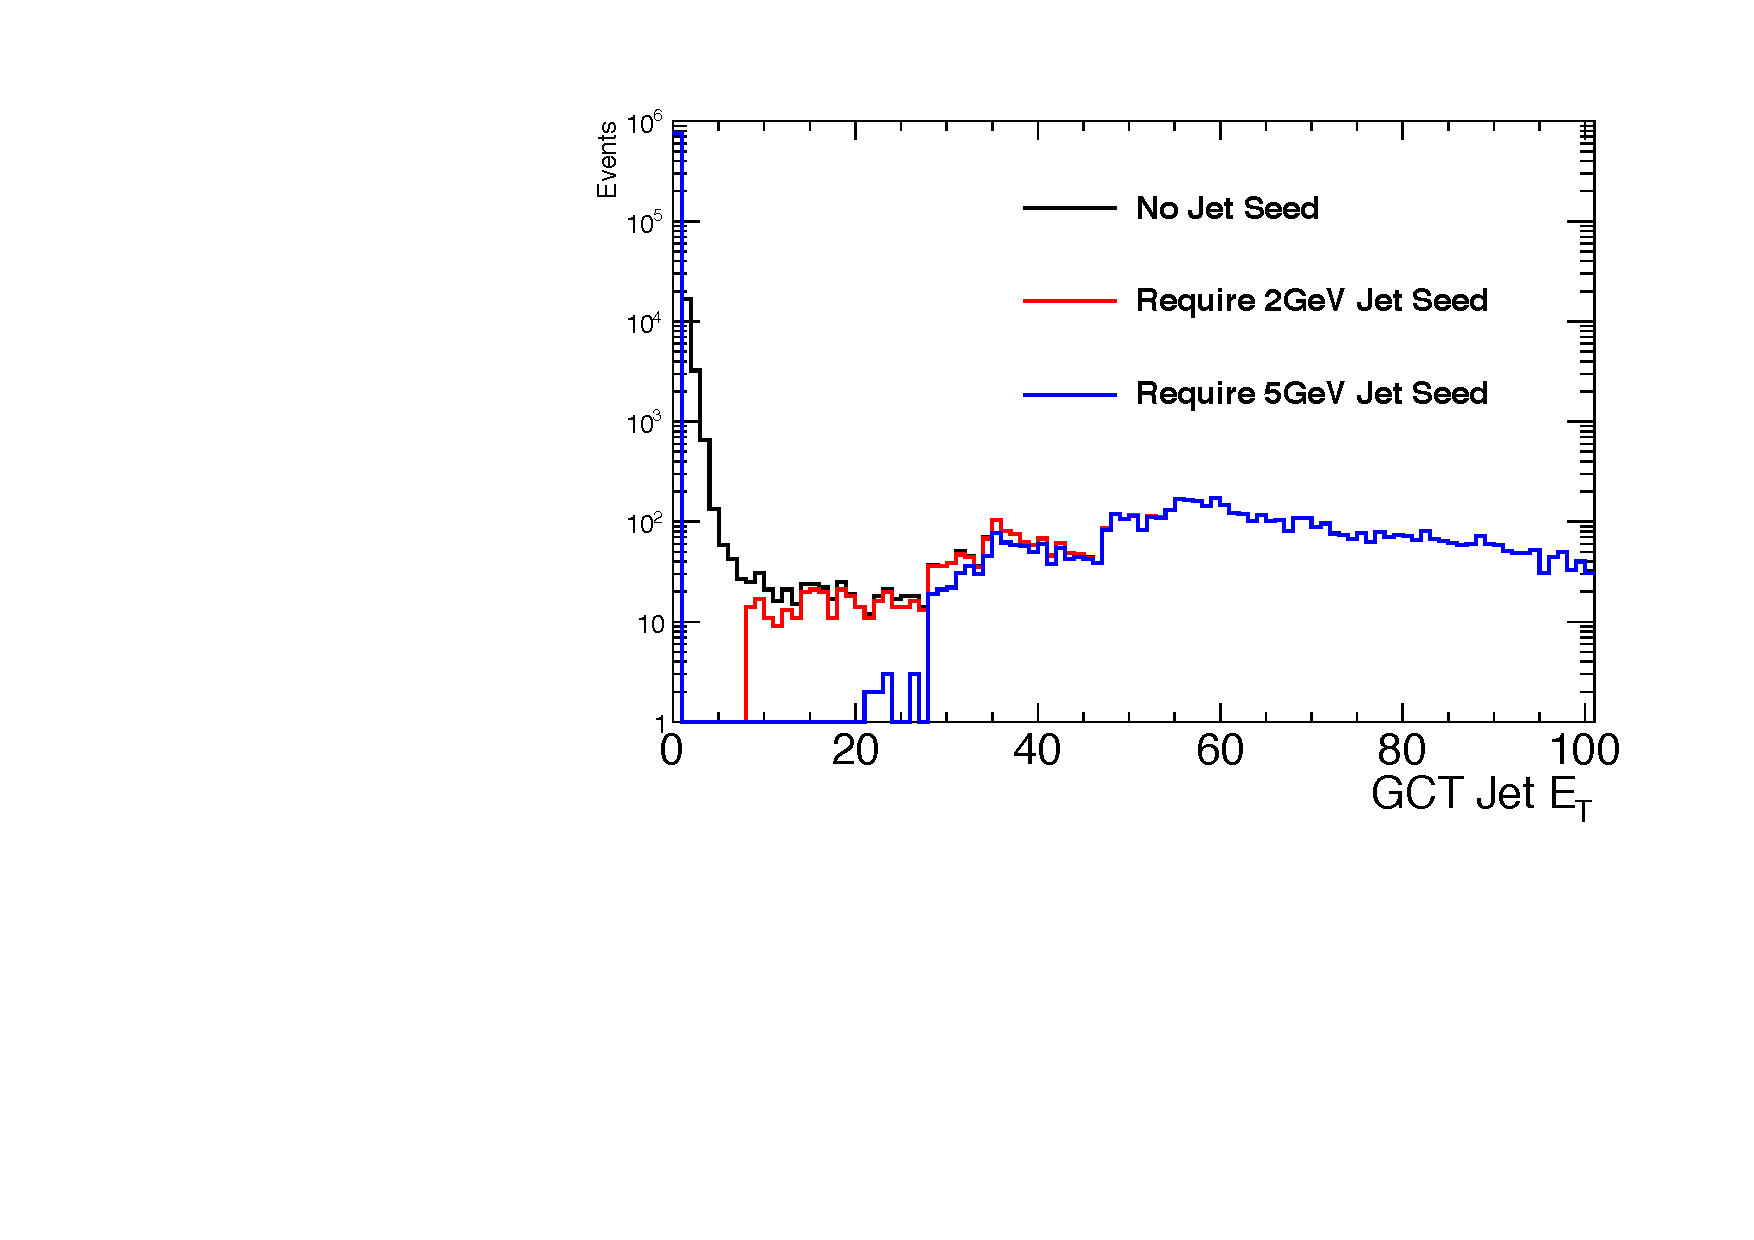
\includegraphics[width=0.45\textwidth]{generated/LoneTrigger/GCT_Jet_Rank_highPU.pdf}
     }
    \subfigure[Efficiency of applying a requirement of 2 or 5 \GeV with respect to no requirement.]{
          \label{fig:GCTrankRatio}
          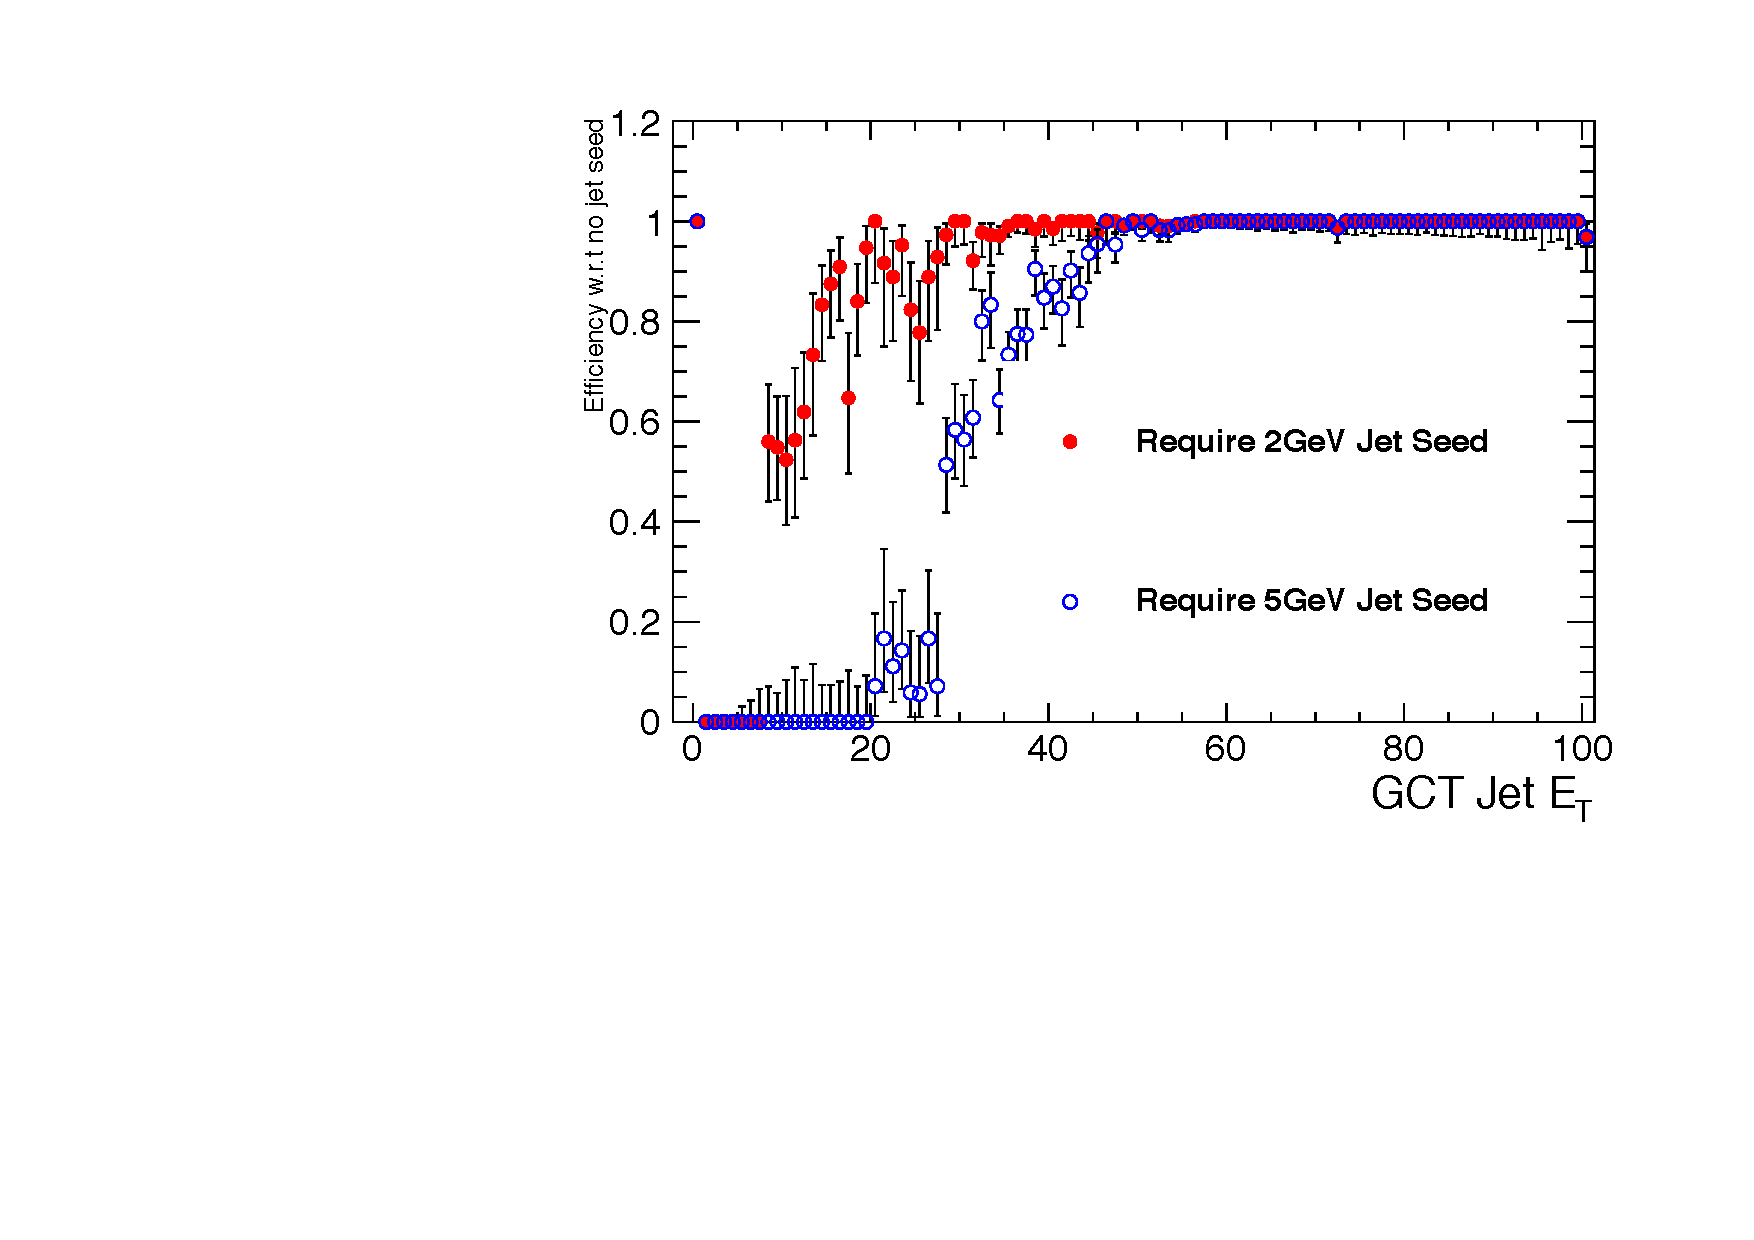
\includegraphics[width=0.45\textwidth]{generated/LoneTrigger/GCT_Jet_Rank_highPU_ratio.pdf}
     }
    \caption{Effect of requiring a jet seed threshold on GCT internal jets.}
    \label{fig:GCTrank}
\end{figure}


Figure~\ref{fig:GCTrank} shows how the different threshold requirements effect the rank of the internal GCT jets.
The effect is to remove all jets below 2(5)\GeV and to cut out jets from the low end of the distribution. 
From Figure~\ref{fig:GCTrankRatio} it is possible to see the point beyond which the requirement of a jet seed has no effect. 
For a cut of 2 \GeV jets above a rank of $\approx$ 35 are not effected, for a seed threshold of 5 \GeV jets above a 
rank of 55 are not effected.


% section gct_hadronic_triggers (end)

% chapter level_one_trigger (end)